%==============================================================
%  EE201 -- Circuit Theory I
%  Lecture 8 : Planar Graphs, the Mesh Matrix and Mesh Currents -- slides
%  M. Mert Ankaralı, METU EEE
%
%  Compile:  ./build.sh      (or: pdflatex EE201_Lecture_8_slides.tex, twice)
%  Same colour code as the handout:
%      charge = purple, current = blue, voltage = orange, power = green
%==============================================================
\documentclass[11pt,aspectratio=169]{beamer}

\usepackage[T1]{fontenc}
\usepackage[utf8]{inputenc}
\usepackage[english]{babel}
\usepackage{lmodern}
\usepackage{amsmath,amssymb}
\usepackage{booktabs}
\usepackage{array}
\usepackage{colortbl}
\usepackage{tikz}
\usepackage[american,siunitx]{circuitikz}
\usetikzlibrary{matrix,arrows.meta,positioning,calc,decorations.pathreplacing,decorations.pathmorphing,decorations.markings}
\usetikzlibrary{overlay-beamer-styles}

%-------------------- plain METU-flavoured theme --------------
\usetheme{default}
\usecolortheme{default}
\useinnertheme{rectangles}
\setbeamertemplate{navigation symbols}{}
\setbeamertemplate{itemize items}[square]
\setbeamerfont{frametitle}{size=\large,series=\bfseries}
\setbeamerfont{title}{size=\LARGE,series=\bfseries}

\definecolor{metured}{RGB}{155,27,48}
\definecolor{metugray}{RGB}{88,89,91}
\definecolor{metulight}{RGB}{243,240,241}
\definecolor{ccur}{RGB}{0,102,170}
\definecolor{cvolt}{RGB}{214,120,0}
\definecolor{cpow}{RGB}{23,128,74}
\definecolor{ccharge}{RGB}{124,60,160}
\definecolor{cflux}{RGB}{0,138,138}
\definecolor{copper}{RGB}{184,98,30}

\setbeamercolor{structure}{fg=metured}
\setbeamercolor{frametitle}{fg=metured,bg=}
\setbeamercolor{title}{fg=metured}
\setbeamercolor{normal text}{fg=black!88}
\setbeamercolor{block title}{fg=white,bg=metured}
\setbeamercolor{block body}{bg=metulight}
\setbeamercolor{alerted text}{fg=metured}

\setbeamertemplate{frametitle}{%
  \vspace{0.55em}%
  \usebeamerfont{frametitle}\usebeamercolor[fg]{frametitle}\insertframetitle\par
  \vspace{-0.2em}{\color{metured}\rule{\textwidth}{1pt}}\par\vspace{-0.2em}}

\setbeamertemplate{footline}{%
  \hbox{\begin{beamercolorbox}[wd=\paperwidth,ht=2.4ex,dp=1.4ex,leftskip=1.2em,rightskip=1.2em]{}%
  \tiny\color{metugray}\coursecode\ \textbar\ Lecture 8: Planar Graphs, the Mesh Matrix and Mesh Currents
  \hfill \insertframenumber/\inserttotalframenumber
  \end{beamercolorbox}}}

%-------------------- macros ----------------------------------
\newcommand{\coursecode}{EE201}
\newcommand{\term}{Fall 2026--2027}
\newcommand{\Icol}[1]{\textcolor{ccur}{#1}}
\newcommand{\Vcol}[1]{\textcolor{cvolt}{#1}}
\newcommand{\Pcol}[1]{\textcolor{cpow}{#1}}
\newcommand{\Qcol}[1]{\textcolor{ccharge}{#1}}
\newcommand{\Fcol}[1]{\textcolor{cflux}{#1}}
\newcommand{\uni}[1]{\,\mathrm{#1}}
\newcommand{\A}{\uni{A}} \newcommand{\V}{\uni{V}}
\newcommand{\W}{\uni{W}} \newcommand{\J}{\uni{J}}
\newcommand{\Cb}{\uni{C}} \newcommand{\s}{\uni{s}}
\newcommand{\Wb}{\uni{Wb}} \newcommand{\Hy}{\uni{H}}
\newcommand{\Sie}{\uni{S}}


\ctikzset{bipoles/length=0.9cm, label/align=straight,
          bipoles/generic/height=0.28, bipoles/generic/width=0.62}
\tikzset{
  iar/.style={-{Stealth[length=2.2mm]}, ccur, thick},
  glab/.style={font=\footnotesize, text=metured},
  ttl/.style={font=\scriptsize\bfseries, text=metugray},
  capn/.style={font=\scriptsize, text=metugray, align=center},
  pol/.style={font=\small, text=cvolt},
  nlab/.style={circle, draw=metured, text=metured, font=\scriptsize, inner sep=0.7pt},
  blab/.style={font=\footnotesize, text=black!80},
  gbr/.style={black!75, thick, postaction={decorate, decoration={markings,
      mark=at position 0.56 with {\arrow{Stealth[length=2.5mm]}}}}},
  hal/.style={draw=cpow!60, line width=6pt, opacity=0.35, line cap=round, line join=round},
  halo/.style={circle, fill=metured!16, minimum size=0.95cm},
  elem/.style={draw=metugray, thick, fill=metulight},
  bigarr/.style={-{Stealth[length=3mm]}, very thick, metugray},
}

\newcommand{\nd}[1]{\tikz[baseline=(c.base)]\node[nlab](c){#1};}
\newcommand{\brarr}[4]{%
  \draw[iar] ($(#1)!0.34!(#2)!0.34cm!#3:(#2)$) -- ($(#1)!0.66!(#2)!0.34cm!#3:(#2)$);
  \node[blab] at ($(#1)!0.5!(#2)!0.66cm!#3:(#2)$) {#4};}
\newcommand{\gbranch}[4]{%
  \draw[gbr] (#1) -- (#2);
  \node[blab] at ($(#1)!0.5!(#2)!0.28cm!#3:(#2)$) {#4};}
%  An incidence matrix with node labels on the left and branch numbers on top.
%  #1 name, #2 number of columns, #3 node labels, #4 rows (entries separated by \&),
%  #5 extra TikZ code drawn on top (may refer to the cells #1-i-j)
\newcommand{\incmat}[5]{%
  \begin{tikzpicture}[baseline={([yshift=-0.6ex]#1.center)}]
    \matrix (#1) [matrix of math nodes, ampersand replacement=\&,
                  left delimiter={[}, right delimiter={]}, inner sep=1pt,
                  column sep=0.45em,
                  nodes={text width=1.35em, align=right, minimum height=1.25em,
                         inner sep=1pt}] {#4};
    \foreach \j in {1,...,#2}
      \node[font=\scriptsize, text=metugray, anchor=south east, inner sep=1pt]
        at ([yshift=2pt]#1-1-\j.north east) {\j};
    \foreach \lab [count=\i] in {#3}
      \node[nlab, left=11pt] at (#1.west |- #1-\i-1) {\lab};
    #5
  \end{tikzpicture}}
\newcommand{\xfmr}[2]{%
  \begin{scope}[xshift=#1 cm]
    \ctikzset{bipoles/length=1.35cm}
    \draw (0,0) to[L] (0,#2);
    \draw (1.6,#2) to[L] (1.6,0);
    \draw[line width=1.1pt, metugray] (0.72,-0.05) -- (0.72,#2+0.05);
    \draw[line width=1.1pt, metugray] (0.88,-0.05) -- (0.88,#2+0.05);
    \fill (0.36,#2-0.2) circle (2.1pt);
    \fill (1.24,#2-0.2) circle (2.1pt);
  \end{scope}}
%  Same, with explicit column labels: #1 name, #2 column labels, #3 row labels,
%  #4 rows, #5 extra TikZ code
\newcommand{\incmatc}[5]{%
  \begin{tikzpicture}[baseline={([yshift=-0.6ex]#1.center)}]
    \matrix (#1) [matrix of math nodes, ampersand replacement=\&,
                  left delimiter={[}, right delimiter={]}, inner sep=1pt,
                  column sep=0.45em,
                  nodes={text width=1.35em, align=right, minimum height=1.25em,
                         inner sep=1pt}] {#4};
    \foreach \lab [count=\j] in {#2}
      \node[font=\scriptsize, text=metugray, anchor=south east, inner sep=1pt]
        at ([yshift=2pt]#1-1-\j.north east) {\lab};
    \foreach \lab [count=\i] in {#3}
      \node[nlab, left=11pt] at (#1.west |- #1-\i-1) {\lab};
    #5
  \end{tikzpicture}}
\newcommand{\bridgecoords}{%
  \coordinate (n1) at (0,1.7);  \coordinate (n2) at (-1.5,0);
  \coordinate (n3) at (1.5,0);  \coordinate (n4) at (0,-1.7);}
\newcommand{\bridgenodes}{%
  \foreach \k/\pos in {1/above, 2/left, 3/right, 4/below}
    {\fill[metured] (n\k) circle (2.2pt); \node[nlab, \pos=3pt] at (n\k) {\k};}}
\newcommand{\bridgecircuit}{%
  \draw (n1) to[generic] (n2);  \draw (n1) to[generic] (n3);
  \draw (n3) to[generic] (n2);  \draw (n2) to[generic] (n4);
  \draw (n3) to[generic] (n4);
  \coordinate (s6) at (-2.6,-1.7); \coordinate (e6) at (-2.6,1.7);
  \draw (n4) -- (s6) to[generic] (e6) -- (n1);}
\newcommand{\bridgegraph}{%
  \gbranch{n1}{n2}{-90}{1}  \gbranch{n1}{n3}{90}{2}  \gbranch{n3}{n2}{-90}{3}
  \gbranch{n2}{n4}{-90}{4}  \gbranch{n3}{n4}{90}{5}
  \draw[gbr] (n4) to[out=180, in=180, looseness=2.3] (n1);
  \node[blab] at (-2.55,0) {6};
  \bridgenodes}
%  A graph branch from #1 to #2 with its branch voltage: + near the tail, - near the head,
%  v_#4 in the middle; #3 = auto=left or auto=right picks the side
\newcommand{\gvbranch}[4]{%
  \draw[gbr] (#1) --
    node[pos=0.27, #3, pol, inner sep=1pt] {$+$}
    node[pos=0.5, #3, font=\small, text=cvolt, inner sep=2.5pt] {$v_{#4}$}
    node[pos=0.73, #3, pol, inner sep=1pt] {$-$} (#2);}
\newcommand{\bridgevgraph}{%
  \gvbranch{n1}{n2}{auto=right}{1}  \gvbranch{n1}{n3}{auto=left}{2}
  \gvbranch{n3}{n2}{auto=right}{3}  \gvbranch{n2}{n4}{auto=right}{4}
  \gvbranch{n3}{n4}{auto=left}{5}
  \draw[gbr] (n4) to[out=180, in=180, looseness=2.3]
    node[pos=0.22, left, pol, inner sep=2pt] {$+$}
    node[pos=0.5, left, font=\small, text=cvolt] {$v_6$}
    node[pos=0.78, left, pol, inner sep=2pt] {$-$} (n1);
  \bridgenodes}
%  One branch, for the definition: + at the tail, - at the head, current along the arrow
\newcommand{\onebranch}{%
  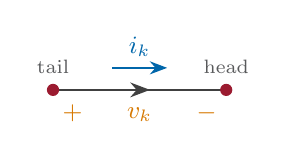
\begin{tikzpicture}[baseline=-0.6ex]
    \coordinate (p) at (0,0); \coordinate (q) at (2.2,0);
    \draw[gbr] (p) -- (q);
    \fill[metured] (p) circle (2.2pt); \fill[metured] (q) circle (2.2pt);
    \node[pol] at (0.25,-0.3) {$+$}; \node[pol] at (1.95,-0.3) {$-$};
    \node[font=\small, text=cvolt] at (1.1,-0.32) {$v_k$};
    \draw[iar] (0.75,0.28) -- (1.45,0.28); \node[font=\small, text=ccur] at (1.1,0.55) {$i_k$};
    \node[font=\scriptsize, text=metugray] at (0,0.3) {tail};
    \node[font=\scriptsize, text=metugray] at (2.2,0.3) {head};
  \end{tikzpicture}}
\newcommand{\U}[2]{\uncover<#1->{#2}}
\providecommand{\ohm}{\,\Omega}

\hypersetup{colorlinks=true,allcolors=metured}

\title{Lecture 8: Planar Graphs,\\ the Mesh Matrix and Mesh Currents}
\subtitle{EE201 -- Circuit Theory I}
\author{M. Mert Ankaralı}
\institute{\small Department of Electrical and Electronics Engineering\\
           Middle East Technical University}
\date{}

%==============================================================
%-------------------- Lecture 8 additions ---------------------
\tikzset{mlabst/.style={draw=ccur, text=ccur, fill=white, rounded corners=1.5pt,
                        inner sep=1.2pt, font=\scriptsize\bfseries}}
%  A boxed mesh number, for the text
\newcommand{\mlab}[1]{\tikz[baseline=(c.base)]\node[mlabst](c){#1};}
%  A clockwise mesh arrow at (#2,#3) with mesh number #4; optional radius #1
\newcommand{\meshcw}[4][0.32]{%
  \draw[ccur, thick, -{Stealth[length=2mm]}] ($(#2,#3)+(150:#1)$)
    arc[start angle=150, end angle=-150, radius=#1];
  \node[mlabst] at (#2,#3) {#4};}
%  The three inner meshes of the bridge graph (after \bridgecoords)
\newcommand{\bridgemeshes}{%
  \meshcw[0.3]{0}{0.82}{1} \meshcw[0.3]{0}{-0.78}{2} \meshcw[0.24]{-1.55}{0.66}{3}}
\newcommand{\fillmeshA}[1][]{\fill[ccur!14, #1] (n1) -- (n2) -- (n3) -- cycle;}
\newcommand{\fillmeshB}[1][]{\fill[ccur!14, #1] (n2) -- (n3) -- (n4) -- cycle;}
\newcommand{\fillmeshC}[1][]{\fill[ccur!14, #1] (n4) to[out=180, in=180, looseness=2.3] (n1) -- (n2) -- cycle;}
%  The bridge graph drawn as a square: both diagonals cross
%  Separable / nonseparable pictures: before and after removing one node.
%  Removed node: open grey circle; removed branches: dashed grey.
\tikzset{gone/.style={gray!55, thick, dash pattern=on 2.5pt off 2pt},
  gonenode/.style={gray!70, thick, fill=white},
  gonelab/.style={nlab, draw=gray!70, text=gray!70}}
\newcommand{\twotricoords}{%
  \coordinate (c) at (1.6,0.8);
  \coordinate (a1) at (0,1.6); \coordinate (a2) at (0,0);
  \coordinate (b1) at (3.2,1.6); \coordinate (b2) at (3.2,0);}
\newcommand{\twotri}{%
  \twotricoords
  \draw[black!75, thick] (c) -- (a1) -- (a2) -- cycle;
  \draw[black!75, thick] (c) -- (b1) -- (b2) -- cycle;
  \foreach \p in {a1,a2,b1,b2,c} \fill[metured] (\p) circle (2.2pt);}
\newcommand{\twotricut}{%
  \twotricoords
  \draw[gone] (a1) -- (c) -- (a2);  \draw[gone] (b1) -- (c) -- (b2);
  \draw[cvolt, very thick] (a1) -- (a2);  \draw[ccur, very thick] (b1) -- (b2);
  \foreach \p in {a1,a2,b1,b2} \fill[metured] (\p) circle (2.2pt);
  \draw[gonenode] (c) circle (2.6pt);}
%  N with node 2 removed: branches 1, 3, 4 go; 2, 5, 6 stay (one piece)
\newcommand{\bridgecut}{%
  \bridgecoords
  \draw[gone] (n1) -- (n2);  \draw[gone] (n3) -- (n2);  \draw[gone] (n2) -- (n4);
  \begin{scope}[gbr/.append style={ccur, very thick}]
    \gbranch{n1}{n3}{90}{2}  \gbranch{n3}{n4}{90}{5}
    \draw[gbr] (n4) to[out=180, in=180, looseness=2.3] (n1);
  \end{scope}
  \node[blab] at (-2.55,0) {6};
  \foreach \k/\pos in {1/above, 3/right, 4/below}
    {\fill[metured] (n\k) circle (2.2pt); \node[nlab, \pos=3pt] at (n\k) {\k};}
  \draw[gonenode] (n2) circle (2.6pt);
  \node[gonelab, left=3pt] at (n2) {2};}
%  Separable vs nonseparable, before and after removing a node. #1, #3: extra options
%  for the two "after" pictures; #2, #4: for the removed parts drawn in them
%  (overlay styles on slides, empty in the notes)
\newcommand{\nsepfigure}[4]{%
  \begin{tikzpicture}[scale=0.8]
    \begin{scope}
      \twotri
      \node[ttl] at (1.6,-1.2) {separable};
    \end{scope}
    \begin{scope}[#1]
      \draw[bigarr] (3.6,0.8) -- (4.4,0.8);
      \node[capn] at (4.0,1.35) {remove\\ centre};
      \begin{scope}[xshift=4.8cm, gone/.append style={#2}, gonenode/.append style={#2}]
        \twotricut
      \end{scope}
      \node[ttl] at (6.4,-1.2) {\textcolor{cvolt}{two} \textcolor{ccur}{pieces}};
    \end{scope}
    \draw[metugray!50] (8.7,-1.4) -- (8.7,2.3);
    \begin{scope}[xshift=11.0cm, yshift=0.8cm, scale=0.75, transform shape]
      \bridgecoords \bridgegraph
    \end{scope}
    \node[ttl] at (10.6,-1.2) {nonseparable ($\mathcal{N}$)};
    \begin{scope}[#3]
      \draw[bigarr] (12.55,0.8) -- (13.45,0.8);
      \node[capn] at (13.0,1.35) {remove\\ node 2};
      \begin{scope}[xshift=15.9cm, yshift=0.8cm, scale=0.75, transform shape,
                    gone/.append style={#4}, gonenode/.append style={#4},
                    gonelab/.append style={#4}]
        \bridgecut
      \end{scope}
      \node[ttl] at (15.5,-1.2) {\textcolor{ccur}{still one piece}};
    \end{scope}
  \end{tikzpicture}}
\newcommand{\squarekfour}{%
  \coordinate (s1) at (0,2); \coordinate (s3) at (2,2);
  \coordinate (s4) at (2,0); \coordinate (s2) at (0,0);
  \foreach \u/\v/\k/\lp in {s1/s2/1/left, s1/s3/2/above, s2/s4/4/below, s3/s4/5/right}
    \draw[black!75, thick] (\u) -- (\v) node[midway, \lp, blab] {\k};
  \draw[black!75, thick] (s3) -- (s2) node[pos=0.25, above left, blab, inner sep=1pt] {3};
  \draw[black!75, thick] (s4) -- (s1) node[pos=0.25, above right, blab, inner sep=1pt] {6};
  \foreach \k/\pos in {1/above left, 2/below left, 3/above right, 4/below right}
    {\fill[metured] (s\k) circle (2.2pt); \node[nlab, \pos=1pt] at (s\k) {\k};}}
%  The circuit of the Tellegen example (10 V, 2, 4, 12 ohm), with current references
%  A hop (bump): the wire passes over another one without touching it.
%  \hopseg{P}{X}{Q}: from P to Q, jumping at the crossing point X
\newcommand{\hopr}{0.22cm}
\newcommand{\hopseg}[3]{%
  ($(#2)!\hopr!(#1)$) to[bend left=90, looseness=1.55] ($(#2)!\hopr!(#3)$)}
%  The square drawing of the bridge graph, branch 6 hopping over branch 3
\newcommand{\squarehop}{%
  \coordinate (s1) at (0,2); \coordinate (s3) at (2,2);
  \coordinate (s4) at (2,0); \coordinate (s2) at (0,0);
  \coordinate (sx) at (1,1);
  \foreach \u/\v/\k/\lp in {s1/s2/1/left, s1/s3/2/above, s2/s4/4/below, s3/s4/5/right}
    \draw[black!75, thick] (\u) -- (\v) node[midway, \lp, blab] {\k};
  \draw[black!75, thick] (s3) -- (s2) node[pos=0.25, above left, blab, inner sep=1pt] {3};
  \draw[copper, very thick] (s4) -- \hopseg{s4}{sx}{s1} -- (s1);
  \node[blab, text=copper] at (1.62,0.62) {6};
  \foreach \k/\pos in {1/above left, 2/below left, 3/above right, 4/below right}
    {\fill[metured] (s\k) circle (2.2pt); \node[nlab, \pos=1pt] at (s\k) {\k};}}
%  The nonplanar hexagon graph with as few hops as possible: one diagonal goes around
%  the outside, and one hop is still left
\newcommand{\hexhop}{%
  \foreach \a/\n in {0/a,60/b,120/c,180/d,240/e,300/f} \coordinate (\n) at (\a:1.15);
  \draw[black!75, thick] (a) -- (b) -- (c) -- (d) -- (e) -- (f) -- cycle;
  \draw[black!75, thick] (a) -- (d);
  \draw[black!75, thick] (b) .. controls (3.1,2.2) and (0.6,-3.3) .. (e);
  \draw[copper, very thick] (c) -- \hopseg{c}{0,0}{f} -- (f);
  \foreach \n in {a,b,c,d,e,f} \fill[metured] (\n) circle (2.2pt);}
%  The same graph in 3D: hexagon on a board, diagonals lifted to different heights.
%  #1: the x, y, z unit vectors of the view
\newcommand{\hexthreeD}[1]{%
  \begin{scope}[#1]
    \fill[metulight] (-1.55,-1.55,0) -- (1.55,-1.55,0) -- (1.55,1.55,0) -- (-1.55,1.55,0) -- cycle;
    \draw[gray!45] (-1.55,-1.55,0) -- (1.55,-1.55,0) -- (1.55,1.55,0) -- (-1.55,1.55,0) -- cycle;
    \foreach \a in {0,60,...,300}
      \draw[black!75, thick] ({1.15*cos(\a)},{1.15*sin(\a)},0) -- ({1.15*cos(\a+60)},{1.15*sin(\a+60)},0);
    \draw[black!75, thick] ({1.15*cos(120)},{1.15*sin(120)},0) -- ({-1.15*cos(120)},{-1.15*sin(120)},0);
    \foreach \a/\h in {0/0.6, 60/1.15}
      \draw[copper, very thick] plot[domain=0:1, samples=31, variable=\t]
        ({1.15*cos(\a)*(1-2*\t)},{1.15*sin(\a)*(1-2*\t)},{\h*sin(180*\t)});
    \foreach \a in {0,60,...,300} \fill[metured] ({1.15*cos(\a)},{1.15*sin(\a)},0) circle (2.2pt);
  \end{scope}}
\tikzset{
  view top/.style={x={(1cm,0cm)}, y={(0cm,1cm)}, z={(0cm,0cm)}},
  view oblique/.style={x={(0.9cm,-0.32cm)}, y={(0.9cm,0.32cm)}, z={(0cm,0.95cm)}},
  view side/.style={x={(1cm,0cm)}, y={(0.22cm,0.1cm)}, z={(0cm,0.95cm)}},
}
\newcommand{\tcircuit}[1]{%
\begin{tikzpicture}[scale=#1]
  \draw (0,0) to[american voltage source, invert] (0,2.2);
  \node[font=\small, left] at (-0.45,1.1) {$10\V$};
  \draw (0,2.2) to[R] (2.6,2.2);
  \node[font=\small] at (1.3,2.62) {$2\ohm$};
  \draw (2.6,2.2) -- (4.4,2.2);
  \draw (2.6,2.2) to[R] (2.6,0);
  \node[font=\small, right] at (2.85,1.75) {$4\ohm$};
  \draw (4.4,2.2) to[R] (4.4,0);
  \node[font=\small, right] at (4.65,1.1) {$12\ohm$};
  \draw (4.4,0) -- (0,0);
  \draw[iar] (0.55,0.7) -- (0.55,1.5);  \node[font=\small, text=ccur] at (0.85,1.1) {$i_1$};
  \draw[iar] (0.85,1.8) -- (1.75,1.8);  \node[font=\small, text=ccur] at (1.3,1.5) {$i_2$};
  \draw[iar] (2.25,1.45) -- (2.25,0.75); \node[font=\small, text=ccur] at (1.95,1.1) {$i_3$};
  \draw[iar] (4.05,1.45) -- (4.05,0.75); \node[font=\small, text=ccur] at (3.75,1.1) {$i_4$};
  \foreach \x/\y/\k/\pos in {0/2.2/1/above left, 2.6/2.2/2/above, 1.3/0/3/below}
    {\fill[metured] (\x,\y) circle (2.2pt); \node[nlab, \pos=2pt] at (\x,\y) {\k};}
  \meshcw[0.28]{1.3}{0.65}{1}
  \meshcw[0.28]{3.3}{0.6}{2}
\end{tikzpicture}}
%  A mesh matrix: like \incmat, with mesh numbers as row labels
\newcommand{\incmatm}[4]{%
  \begin{tikzpicture}[baseline={([yshift=-0.6ex]#1.center)}]
    \matrix (#1) [matrix of math nodes, ampersand replacement=\&,
                  left delimiter={[}, right delimiter={]}, inner sep=1pt,
                  column sep=0.45em,
                  nodes={text width=1.35em, align=right, minimum height=1.25em,
                         inner sep=1pt}] {#4};
    \foreach \j in {1,...,#2}
      \node[font=\scriptsize, text=metugray, anchor=south east, inner sep=1pt]
        at ([yshift=2pt]#1-1-\j.north east) {\j};
    \foreach \lab [count=\i] in {#3}
      \node[mlabst, left=11pt] at (#1.west |- #1-\i-1) {\lab};
  \end{tikzpicture}}
%  Slides only: the mesh matrix of N, row k shown from overlay k+1 on
\newcommand{\incmatmv}[4]{%
  \begin{tikzpicture}[baseline={([yshift=-0.6ex]#1.center)}]
    \matrix (#1) [matrix of math nodes, ampersand replacement=\&,
                  left delimiter={[}, right delimiter={]}, inner sep=1pt,
                  column sep=0.45em,
                  nodes={text width=1.35em, align=right, minimum height=1.25em,
                         inner sep=1pt},
                  row 1/.style={nodes={visible on=<2->}},
                  row 2/.style={nodes={visible on=<3->}},
                  row 3/.style={nodes={visible on=<4->}}] {#4};
    \foreach \j in {1,...,#2}
      \node[font=\scriptsize, text=metugray, anchor=south east, inner sep=1pt]
        at ([yshift=2pt]#1-1-\j.north east) {\j};
    \foreach \lab [count=\i] in {#3}
      \node[mlabst, left=11pt] at (#1.west |- #1-\i-1) {\lab};
  \end{tikzpicture}}

%==============================================================
\begin{document}

%--------------------------------------------------------------
\begin{frame}[plain]
  \titlepage
  \vspace{-1.2em}
  \begin{center}\scriptsize\color{metugray}
    \Icol{$\blacksquare$}~current, meshes \quad \Vcol{$\blacksquare$}~voltage \quad
    \textcolor{metured}{$\blacksquare$}~nodes
  \end{center}
\end{frame}

%--------------------------------------------------------------
\begin{frame}{From nodes to meshes}
  \vfill
  \begin{center}
    Earlier, from the incidence matrix $A$:\\[6pt]
    $A\Icol{\mathbf{i}} = \mathbf{0}$ \ (KCL), \qquad
    $\Vcol{\mathbf{v}} = A^T\Vcol{\mathbf{e}}$ \ (KVL)\\[6pt]
    \small With the $n-1$ node voltages as unknowns, KVL holds automatically; only KCL is left.
  \end{center}
  \vfill
  \onslide<2->
  \begin{block}{Today: the counterpart, from the meshes}
    A \alert{mesh matrix} $M$ with KVL as $M\Vcol{\mathbf{v}} = \mathbf{0}$, and
    \alert{mesh currents} for which KCL holds automatically.\\
    It works for graphs that can be drawn on a plane without crossings.
  \end{block}
  \vfill
\end{frame}

%--------------------------------------------------------------
\begin{frame}{Planar graphs}
  \begin{block}{Planar graph}
    Can be drawn on a plane so that no two branches intersect at a point that is not a node.
  \end{block}
  \vfill
  \begin{center}
  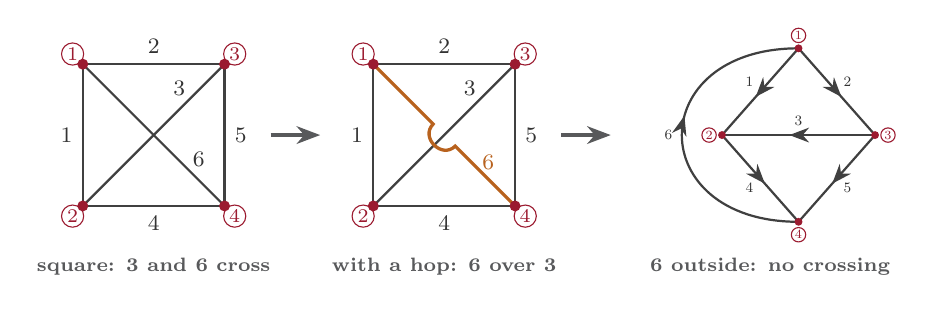
\begin{tikzpicture}[scale=0.9]
    \begin{scope}
      \squarekfour
      \node[ttl] at (1,-0.85) {square: 3 and 6 cross};
    \end{scope}
    \begin{scope}[visible on=<2->]
      \draw[bigarr] (2.65,1) -- (3.35,1);
      \begin{scope}[xshift=4.1cm]
        \squarehop
        \node[ttl] at (1,-0.85) {with a hop: 6 over 3};
      \end{scope}
    \end{scope}
    \begin{scope}[visible on=<3->]
      \draw[bigarr] (6.75,1) -- (7.45,1);
      \begin{scope}[xshift=10.1cm, yshift=1cm, scale=0.72, transform shape]
        \bridgecoords \bridgegraph
      \end{scope}
      \node[ttl] at (9.7,-0.85) {6 outside: no crossing};
    \end{scope}
  \end{tikzpicture}
  \end{center}
  \vfill
  \begin{center}\small
    \only<1>{On paper, branches 3 and 6 seem to cross. Do they meet?}%
    \only<2>{No: two separate wires, the crossing point is \alert{not a node}.\\
      In hardware: a jumper wire, or a track on a second layer of the board.}%
    \only<3->{Redrawn with no crossing (this is $\mathcal{N}$), so the graph is \alert{planar}.\\
      A drawing with crossings does not decide it --- the question is whether
      \emph{some} drawing has none.}
  \end{center}
\end{frame}

%--------------------------------------------------------------
\begin{frame}{A nonplanar graph}
  \vfill
  \begin{center}
  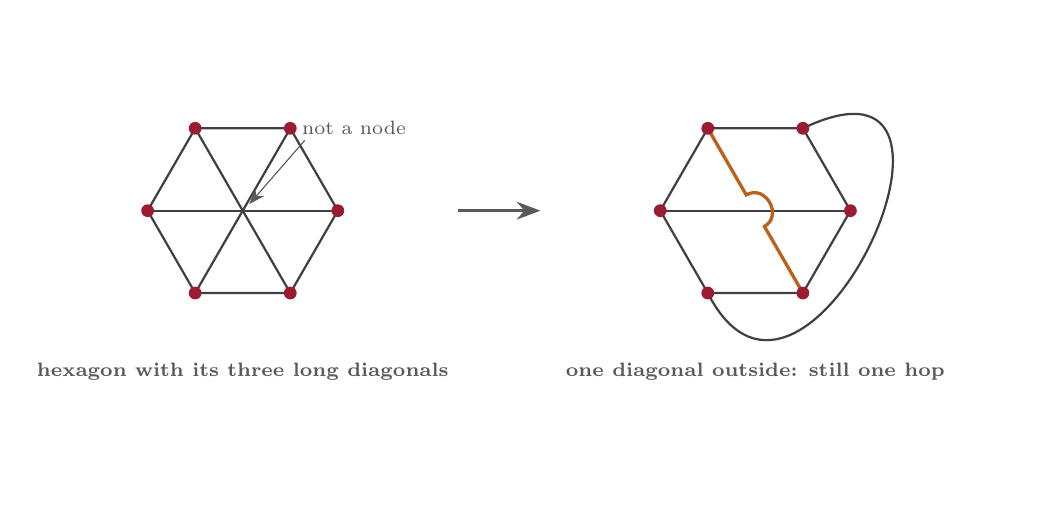
\begin{tikzpicture}[scale=1.05]
    \begin{scope}
      \foreach \a in {0,60,...,300} \coordinate (h\a) at (\a:1.15);
      \draw[black!75, thick] (h0) -- (h60) -- (h120) -- (h180) -- (h240) -- (h300) -- cycle;
      \draw[black!75, thick] (h0) -- (h180); \draw[black!75, thick] (h60) -- (h240);
      \draw[black!75, thick] (h120) -- (h300);
      \foreach \a in {0,60,...,300} \fill[metured] (h\a) circle (2.2pt);
      \draw[-{Stealth[length=2mm]}, metugray] (0.75,0.85) -- (0.08,0.08);
      \node[capn, anchor=south west] at (0.6,0.8) {not a node};
      \node[ttl] at (0,-1.95) {hexagon with its three long diagonals};
    \end{scope}
    \begin{scope}[visible on=<2->]
      \draw[bigarr] (2.6,0) -- (3.6,0);
      \begin{scope}[xshift=6.2cm]
        \hexhop
        \node[ttl] at (0,-1.95) {one diagonal outside: still one hop};
      \end{scope}
    \end{scope}
  \end{tikzpicture}
  \end{center}
  \vfill
  \begin{center}
    \only<1>{Three diagonals cross at the centre. Can the graph be redrawn without crossings?}%
    \only<2->{However it is redrawn, at least one hop remains: \alert{nonplanar}.}
  \end{center}
  \vfill
\end{frame}

%--------------------------------------------------------------
\begin{frame}{A nonplanar graph in 3D}
  \vfill
  \begin{center}
  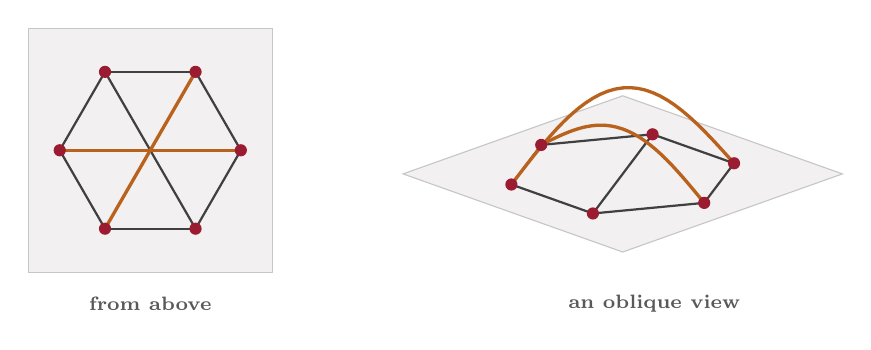
\begin{tikzpicture}[scale=1.0]
    \begin{scope}
      \hexthreeD{view top}
      \node[ttl] at (0,-1.95) {from above};
    \end{scope}
    \begin{scope}[xshift=6.0cm, yshift=-0.3cm, visible on=<2->]
      \hexthreeD{view oblique}
      \node[ttl] at (0.4,-1.65) {an oblique view};
    \end{scope}
  \end{tikzpicture}
  \end{center}
  \vfill
  \begin{center}
    \only<1>{From above it looks like crossings.}%
    \only<2->{Two diagonals are lifted: no two branches meet in space.\\
      A hop is a step into the third dimension --- on a plane, some step is always needed.}
  \end{center}
  \vfill
\end{frame}

%--------------------------------------------------------------
\begin{frame}{Nonseparable graphs}
  \begin{block}{Nonseparable graph}
    A connected graph that stays connected after removing any one node (and the branches
    attached to it).
  \end{block}
  \vfill
  \begin{center}
  \nsepfigure{visible on=<2->}{visible on=<2>}{visible on=<4->}{visible on=<4>}
  \end{center}
  \vfill
  \begin{center}
    \only<-5>{\uncover<5>{Any node of $\mathcal{N}$ can be removed: the rest stays connected.}}%
    \only<6->{From now on: the graph is \alert{planar} and \alert{nonseparable}, drawn without crossings.}
  \end{center}
\end{frame}

%--------------------------------------------------------------
\begin{frame}{Meshes}
  \begin{columns}[c,onlytextwidth]
    \begin{column}{0.42\textwidth}
      \centering
      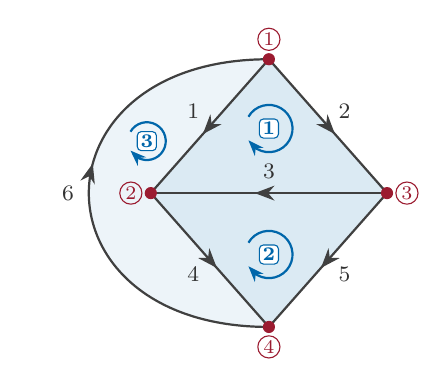
\begin{tikzpicture}[scale=1.0]
        \bridgecoords
        \fillmeshA[visible on=<2->] \fillmeshB[visible on=<2->] \fillmeshC[ccur!7, visible on=<2->]
        \bridgegraph
        \begin{scope}[visible on=<3->] \bridgemeshes \end{scope}
      \end{tikzpicture}
    \end{column}
    \begin{column}{0.56\textwidth}
      A planar drawing divides the plane into regions.\\[4pt]
      \onslide<2->
      \alert{Inner mesh}: the loop around a region inside the graph, with no branch inside
      it. (The outside region is not counted.)\\[6pt]
      \onslide<3->
      \mlab{1}: branches 1, 2, 3 \quad \mlab{2}: 3, 4, 5 \quad \mlab{3}: 1, 4, 6\\[4pt]
      Direction: \alert{clockwise}, by convention.\\[8pt]
      \onslide<4->
      Number of inner meshes: \
      $\ell = b - n + 1 = 6 - 4 + 1 = 3$\\[2pt]
      {\small --- the number of independent KVL equations found earlier.}
    \end{column}
  \end{columns}
\end{frame}

%--------------------------------------------------------------
\begin{frame}{The mesh matrix}
  \vfill
  \begin{block}{Mesh matrix $M$ \ ($\ell \times b$)}
    \[
      m_{jk} =
      \begin{cases}
        +1 & \text{branch } k \text{ in mesh } j, \text{ directions coincide},\\
        -1 & \text{branch } k \text{ in mesh } j, \text{ directions opposite},\\
        \phantom{+}0 & \text{otherwise.}
      \end{cases}
    \]
  \end{block}
  \vfill
  \begin{center}
    A row is a mesh: walk around it clockwise.\\
    Each branch you meet: \alert{$+1$} if its arrow points the way you walk,
    \alert{$-1$} if it points against you.
  \end{center}
  \vfill
\end{frame}

%--------------------------------------------------------------
\begin{frame}{Example: the mesh matrix of $\mathcal{N}$}
  \begin{columns}[c,onlytextwidth]
    \begin{column}{0.38\textwidth}
      \centering
      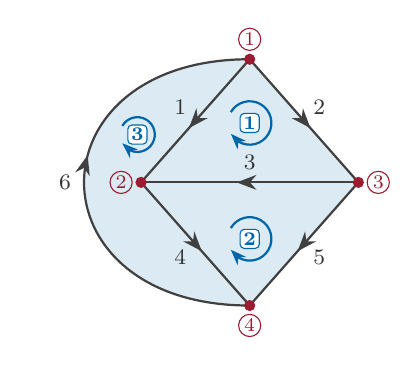
\begin{tikzpicture}[scale=0.92]
        \bridgecoords
        \fillmeshA[visible on=<2>] \fillmeshB[visible on=<3>] \fillmeshC[visible on=<4>]
        \bridgegraph \bridgemeshes
      \end{tikzpicture}
    \end{column}
    \begin{column}{0.6\textwidth}
      \small
      \only<2>{\mlab{1}: \nd1 $\to$ \nd3 $\to$ \nd2 $\to$ \nd1. Branches 2, 3 along: $+1$;
        branch 1 against: $-1$.}%
      \only<3>{\mlab{2}: \nd2 $\to$ \nd3 $\to$ \nd4 $\to$ \nd2. Branch 5 along: $+1$;
        branches 3, 4 against: $-1$.}%
      \only<4>{\mlab{3}: \nd4 $\to$ \nd1 $\to$ \nd2 $\to$ \nd4. Branches 6, 1, 4 all along:
        $+1$.}%
      \only<5->{Three meshes, six branches: $M$ is $3 \times 6$.}
      \[
        M = \incmatmv{Mn}{6}{1,2,3}{%
          -1 \& 1 \& 1 \& 0 \& 0 \& 0\\
           0 \& 0 \& -1 \& -1 \& 1 \& 0\\
           1 \& 0 \& 0 \& 1 \& 0 \& 1\\}
      \]
    \end{column}
  \end{columns}
\end{frame}

%--------------------------------------------------------------
\begin{frame}{KVL with the mesh matrix}
  \vfill
  \begin{center}
  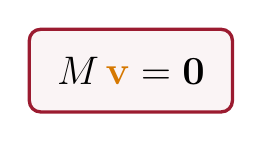
\begin{tikzpicture}
    \node[draw=metured, very thick, rounded corners=4pt, fill=metured!5, inner sep=10pt] {%
      \Large $M\,\Vcol{\mathbf{v}} = \mathbf{0}$};
  \end{tikzpicture}\\[6pt]
  KVL around every mesh, $\Vcol{\mathbf{v}} = [\,\Vcol{v_1}\ \cdots\ \Vcol{v_b}\,]^T$
  \end{center}
  \vfill
  \onslide<2->
  \begin{center}
    For $\mathcal{N}$:\quad
    $-\Vcol{v_1} + \Vcol{v_2} + \Vcol{v_3} = 0, \qquad
     -\Vcol{v_3} - \Vcol{v_4} + \Vcol{v_5} = 0, \qquad
     \Vcol{v_1} + \Vcol{v_4} + \Vcol{v_6} = 0$\\[8pt]
    \small Walking along an arrow goes from $+$ to $-$: that voltage counts with $+$.
  \end{center}
  \vfill
\end{frame}

%--------------------------------------------------------------
\begin{frame}{Mesh currents}
  \begin{columns}[c,onlytextwidth]
    \begin{column}{0.38\textwidth}
      \centering
      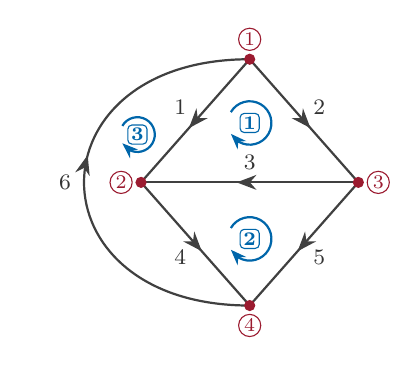
\begin{tikzpicture}[scale=0.92]
        \bridgecoords \bridgegraph \bridgemeshes
      \end{tikzpicture}
    \end{column}
    \begin{column}{0.6\textwidth}
      \begin{block}{Mesh current}
        A current $\Icol{i_{Mk}}$ that circulates around mesh $k$, clockwise.\\
        $\Icol{\mathbf{i}_M} = [\,\Icol{i_{M1}}\ \cdots\ \Icol{i_{M\ell}}\,]^T$
      \end{block}
      \onslide<2->
      A branch carries the mesh currents of its meshes:\\
      $+$ if the mesh goes along its arrow, $-$ if against.\\[6pt]
      \onslide<3->
      Branch 3, in \mlab{1} (along) and \mlab{2} (against):
      \ $\Icol{i_3} = \Icol{i_{M1}} - \Icol{i_{M2}}$\\
      Branch 2, only in \mlab{1}: \ $\Icol{i_2} = \Icol{i_{M1}}$
    \end{column}
  \end{columns}
\end{frame}

%--------------------------------------------------------------
\begin{frame}{Example: branch currents of $\mathcal{N}$ from mesh currents}
  \begin{columns}[c,onlytextwidth]
    \begin{column}{0.3\textwidth}
      \centering
      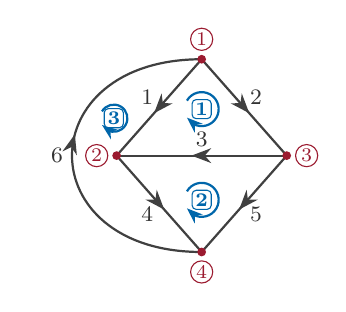
\begin{tikzpicture}[scale=0.72]
        \bridgecoords \bridgegraph \bridgemeshes
      \end{tikzpicture}
    \end{column}
    \begin{column}{0.68\textwidth}
      \[
        \begin{aligned}
          \Icol{i_1} &= \U2{-\Icol{i_{M1}} + \Icol{i_{M3}}} & \Icol{i_4} &= \U2{-\Icol{i_{M2}} + \Icol{i_{M3}}}\\
          \Icol{i_2} &= \U2{\Icol{i_{M1}}}                  & \Icol{i_5} &= \U2{\Icol{i_{M2}}}\\
          \Icol{i_3} &= \U2{\Icol{i_{M1}} - \Icol{i_{M2}}}  & \Icol{i_6} &= \U2{\Icol{i_{M3}}}
        \end{aligned}
      \]
      \onslide<3->
      \[
        \begin{bmatrix}
          \Icol{i_1}\\ \Icol{i_2}\\ \Icol{i_3}\\ \Icol{i_4}\\ \Icol{i_5}\\ \Icol{i_6}
        \end{bmatrix}
        =
        \underbrace{\begin{bmatrix}
          -1 &  0 & 1\\
           1 &  0 & 0\\
           1 & -1 & 0\\
           0 & -1 & 1\\
           0 &  1 & 0\\
           0 &  0 & 1
        \end{bmatrix}}_{\alert<4->{M^T}}
        \begin{bmatrix} \Icol{i_{M1}}\\ \Icol{i_{M2}}\\ \Icol{i_{M3}} \end{bmatrix}
      \]
    \end{column}
  \end{columns}
  \vfill
  \onslide<4->
  \begin{center}\small
    This matrix is $M^T$: its row 1, $[\,{-1}\ \ 0\ \ 1\,]$, is column 1 of $M$ --- and so on.
  \end{center}
\end{frame}

%--------------------------------------------------------------
\begin{frame}[t]{Mesh currents: remarks}
  \begin{columns}[T,onlytextwidth]
    \begin{column}{0.34\textwidth}
      \centering
      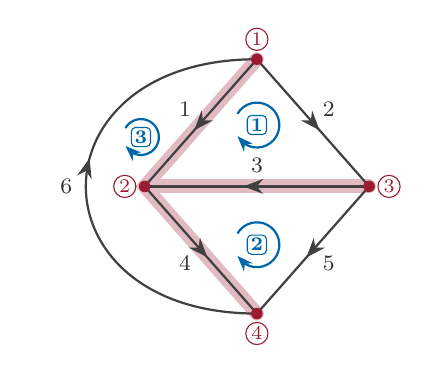
\begin{tikzpicture}[scale=0.95]
        \bridgecoords
        \begin{scope}[visible on=<3->]
          \draw[metured!30, line width=5pt, line cap=round] (n1) -- (n2) -- (n4);
          \draw[metured!30, line width=5pt, line cap=round] (n3) -- (n2);
        \end{scope}
        \bridgegraph
        \bridgemeshes
      \end{tikzpicture}\\[4pt]
      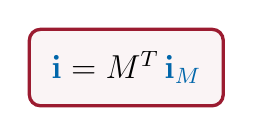
\begin{tikzpicture}
        \node[draw=metured, very thick, rounded corners=4pt, fill=metured!5, inner sep=8pt] {%
          \large $\Icol{\mathbf{i}} = M^T\,\Icol{\mathbf{i}_M}$};
      \end{tikzpicture}
    \end{column}
    \begin{column}{0.64\textwidth}
      \vspace{6pt}
      \begin{itemize}\itemsep8pt
        \item<2-> Know the $\ell$ mesh currents $\Rightarrow$ know all $b$ branch currents.
        \item<3-> KCL puts \alert{no constraint} on $\Icol{\mathbf{i}_M}$. KCL at \nd2:\\[3pt]
              {\small $-\Icol{i_1} - \Icol{i_3} + \Icol{i_4}$\\
              $\;= (\Icol{i_{M1}} - \Icol{i_{M3}}) - (\Icol{i_{M1}} - \Icol{i_{M2}})
               + (-\Icol{i_{M2}} + \Icol{i_{M3}}) = 0$}
        \item<4-> $A\Icol{\mathbf{i}} = AM^T\Icol{\mathbf{i}_M} = \mathbf{0}$ for \alert{every}
              $\Icol{\mathbf{i}_M}$ $\Rightarrow$ \alert{$AM^T = \mathbf{0}$}.
      \end{itemize}
    \end{column}
  \end{columns}
\end{frame}

%--------------------------------------------------------------
\begin{frame}{Rows of $A$ $\perp$ rows of $M$}
  \begin{center}
    $A\Icol{\mathbf{i}} = AM^T\Icol{\mathbf{i}_M} = \mathbf{0}$ for every $\Icol{\mathbf{i}_M}$
    \quad$\Rightarrow$\quad \alert{$AM^T = \mathbf{0}$}
  \end{center}
  \vfill
  \begin{center}
    $A =$\hspace{0.6em}\incmat{Ao}{6}{1,2,3}{%
       1 \&  1 \&  0 \&  0 \&  0 \& -1\\
      -1 \&  0 \& -1 \&  1 \&  0 \&  0\\
       0 \& -1 \&  1 \&  0 \&  1 \&  0\\}{%
      \foreach \i in {1,2,3}
        \node[font=\small, text=metugray, right=6pt] at (Ao.east |- Ao-\i-6) {$\mathbf{a}_\i^T$};
      \draw[metured, thick, rounded corners=2pt, visible on=<2->]
        ([xshift=-2pt]Ao-2-1.north west) rectangle ([xshift=2pt]Ao-2-6.south east);
      \foreach \j in {1,3}
        \draw[cvolt, very thick, visible on=<3->] (Ao-2-\j) circle (0.27);}
    \\[2pt]
    $M =$\hspace{0.6em}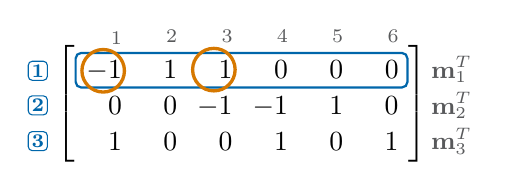
\begin{tikzpicture}[baseline={([yshift=-0.6ex]Mo.center)}]
      \matrix (Mo) [matrix of math nodes, ampersand replacement=\&,
                    left delimiter={[}, right delimiter={]}, inner sep=1pt,
                    column sep=0.45em,
                    nodes={text width=1.35em, align=right, minimum height=1.25em,
                           inner sep=1pt}] {
         -1 \&  1 \&  1 \&  0 \&  0 \&  0\\
          0 \&  0 \& -1 \& -1 \&  1 \&  0\\
          1 \&  0 \&  0 \&  1 \&  0 \&  1\\};
      \foreach \j in {1,...,6}
        \node[font=\scriptsize, text=metugray, anchor=south east, inner sep=1pt]
          at ([yshift=2pt]Mo-1-\j.north east) {\j};
      \foreach \lab [count=\i] in {1,2,3}
        \node[mlabst, left=11pt] at (Mo.west |- Mo-\i-1) {\lab};
      \foreach \i in {1,2,3}
        \node[font=\small, text=metugray, right=6pt] at (Mo.east |- Mo-\i-6) {$\mathbf{m}_\i^T$};
      \draw[ccur, thick, rounded corners=2pt, visible on=<2->]
        ([xshift=-2pt]Mo-1-1.north west) rectangle ([xshift=2pt]Mo-1-6.south east);
      \foreach \j in {1,3}
        \draw[cvolt, very thick, visible on=<3->] (Mo-1-\j) circle (0.27);
    \end{tikzpicture}
  \end{center}
  \vfill
  \begin{center}
    $(AM^T)_{jr} = \mathbf{a}_j^T\mathbf{m}_r = 0$ \ for all $j, r$: \
    \alert{every row of $A$ is orthogonal to every row of $M$}.\\[8pt]
    \onslide<2->{%
    $\mathbf{a}_2^T\mathbf{m}_1 = (-1)(-1) + (0)(1) + (-1)(1) + (1)(0) + (0)(0) + (0)(0) = 0$\\[8pt]}
    \onslide<3->{%
    Node \nd2 and mesh \mlab1 share branches 1 and 3: one term $+1$, one $-1$.}
  \end{center}
  \vfill
\end{frame}

%--------------------------------------------------------------
\begin{frame}{Example: mesh currents in a familiar circuit}
  \begin{center}\small
    Solved earlier with node voltages: $\Icol{i_1} = \Icol{i_2} = 2\A$, $\Icol{i_3} = 1.5\A$,
    $\Icol{i_4} = 0.5\A$, $\Vcol{\mathbf{v}} = [\,{-10}\ \ 4\ \ 6\ \ 6\,]^T\V$.\\
    Write $M$ and check both results with mesh currents.
  \end{center}
  \vspace{-6pt}
  \begin{columns}[c,onlytextwidth]
    \begin{column}{0.46\textwidth}
      \centering
      \tcircuit{0.88}
    \end{column}
    \begin{column}{0.52\textwidth}
      \small
      \onslide<2->{%
      \mlab{1}: up the source, right through $2\ohm$, down the $4\ohm$ --- all along.\\
      \mlab{2}: up the $4\ohm$ (against), down the $12\ohm$ (along).
      \[ M = \begin{bmatrix} 1 & 1 & 1 & 0\\ 0 & 0 & -1 & 1 \end{bmatrix} \]}
      \onslide<3->{%
      $\Icol{i_1} = \Icol{i_2} = \Icol{i_{M1}}$, \ $\Icol{i_3} = \Icol{i_{M1}} - \Icol{i_{M2}}$,
      \ $\Icol{i_4} = \Icol{i_{M2}}$\\[3pt]}
      \onslide<4->{%
      $\Icol{i_{M1}} = 2\A$, $\Icol{i_{M2}} = 0.5\A$ $\Rightarrow$ the same branch currents.\\[3pt]
      KVL: $M\Vcol{\mathbf{v}} = [\,{-10} + 4 + 6,\ \ {-6} + 6\,]^T = \mathbf{0}$}
    \end{column}
  \end{columns}
\end{frame}

%--------------------------------------------------------------
\begin{frame}{Node voltages and mesh currents}
  \vfill
  \begin{center}
  \renewcommand{\arraystretch}{1.35}
  \begin{tabular}{@{}l l l@{}}
  \toprule
   & \textbf{node voltages} & \textbf{mesh currents}\\
  \midrule
  works for                & any connected graph       & planar, nonseparable\\
  number of unknowns       & $n - 1$                   & $\ell = b - n + 1$\\
  matrix                   & $A$ \ ($(n-1)\times b$)   & $M$ \ ($\ell\times b$)\\
  holds automatically      & KVL: $\Vcol{\mathbf{v}} = A^T\Vcol{\mathbf{e}}$
                           & KCL: $\Icol{\mathbf{i}} = M^T\Icol{\mathbf{i}_M}$\\
  left to write            & KCL: $A\Icol{\mathbf{i}} = \mathbf{0}$
                           & KVL: $M\Vcol{\mathbf{v}} = \mathbf{0}$\\
  \bottomrule
  \end{tabular}
  \end{center}
  \vfill
  \begin{center}\small
    And the two matrices fit together: $AM^T = \mathbf{0}$.
  \end{center}
  \vfill
\end{frame}

%--------------------------------------------------------------
\begin{frame}{Looking ahead: why mesh currents?}
  \begin{center}
    Same idea, KCL and KVL swapped: $b$ element, $n-1$ KCL, $\ell$ KVL equations.
  \end{center}
  \vfill
  \begin{center}
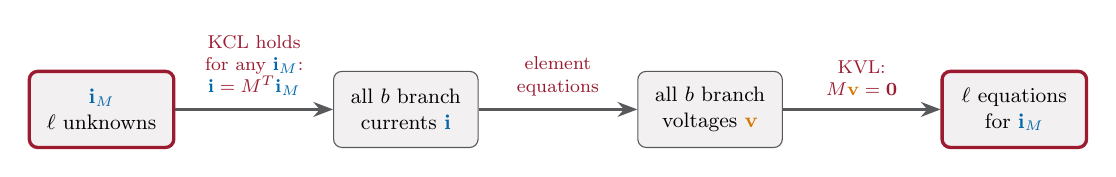
\begin{tikzpicture}[scale=0.84, transform shape,
    fb/.style={draw=metugray, fill=metulight, rounded corners=3pt, align=center,
               minimum height=1.15cm, text width=1.95cm, font=\small},
    fa/.style={-{Stealth[length=2.5mm]}, very thick, metugray},
    fl/.style={font=\footnotesize, align=center, text=metured}]
  \node[fb, draw=metured, very thick] (u) at (0,0) {$\Icol{\mathbf{i}_M}$\\ $\ell$ unknowns};
  \node[fb, visible on=<2->] (a) at (4.6,0) {all $b$ branch\\ currents $\Icol{\mathbf{i}}$};
  \node[fb, visible on=<3->] (b) at (9.2,0) {all $b$ branch\\ voltages $\Vcol{\mathbf{v}}$};
  \node[fb, draw=metured, very thick, visible on=<4->] (c) at (13.8,0) {$\ell$ equations\\ for $\Icol{\mathbf{i}_M}$};
  \draw[fa, visible on=<2->] (u) -- node[fl, above=2pt] {KCL holds\\ for any $\Icol{\mathbf{i}_M}$:\\ $\Icol{\mathbf{i}} = M^T\Icol{\mathbf{i}_M}$} (a);
  \draw[fa, visible on=<3->] (a) -- node[fl, above=2pt] {element\\ equations} (b);
  \draw[fa, visible on=<4->] (b) -- node[fl, above=2pt] {KVL:\\ $M\Vcol{\mathbf{v}} = \mathbf{0}$} (c);
\end{tikzpicture}
  \end{center}
  \vfill
  \onslide<5->
  \begin{center}
    $2b$ unknowns $\to$ \alert{$\ell = b - n + 1 < b$}. \ Fewer: $n-1$ or $\ell$?
    It depends on the circuit.\\[4pt]
    \alert{Mesh analysis} --- coming soon.
  \end{center}
\end{frame}

%--------------------------------------------------------------
\begin{frame}{Summary}
  \vfill
  \begin{itemize}\itemsep5pt
    \item \textbf{Planar}: can be drawn with no crossings. \textbf{Nonseparable}: removing
          any one node leaves it connected.
    \item \textbf{Inner meshes}, clockwise: $\ell = b - n + 1$ of them.
    \item \textbf{Mesh matrix} $M$ ($\ell \times b$): $+1$ along, $-1$ against.
          KVL: $M\Vcol{\mathbf{v}} = \mathbf{0}$.
    \item \textbf{Mesh currents}: $\Icol{\mathbf{i}} = M^T\Icol{\mathbf{i}_M}$. No constraint
          from KCL, so $AM^T = \mathbf{0}$.
    \item \textbf{Why}: with $\Icol{\mathbf{i}_M}$ as unknowns KCL holds automatically; $\ell$
          unknowns are enough --- the idea of mesh analysis.
  \end{itemize}
  \vfill
\end{frame}

%--------------------------------------------------------------
\begin{frame}{Next lecture}
  \vfill
  \begin{center}
  \begin{block}{Nonplanar circuits}
    \alert{Trees}, \alert{cutsets} and fundamental cutsets --- tools that work for any
    connected graph.
  \end{block}
  \end{center}
  \vfill
  \begin{center}
    {\Large\color{metured} Questions?}
  \end{center}
  \vfill
\end{frame}

\end{document}
